%%%%%%%%%%%%%%%%%%%%%%%%%%%%%%%%%%%%%%%%%%%%%%%%%%%%%%%%%%%%%%%%%%%%%%%%%%%
%
% Generic template for TFC/TFM/TFG/Tesis
%
% $Id: estudioTeorico.tex,v 1.4 2014/12/09 11:55:53 macias Exp $
%
% By:
%  + Javier Mac�as-Guarasa. 
%    Departamento de Electr�nica
%    Universidad de Alcal�
%  + Roberto Barra-Chicote. 
%    Departamento de Ingenier�a Electr�nica
%    Universidad Polit�cnica de Madrid   
% 
% Based on original sources by Roberto Barra, Manuel Oca�a, Jes�s Nuevo,
% Pedro Revenga, Fernando Herr�nz and Noelia Hern�ndez. Thanks a lot to
% all of them, and to the many anonymous contributors found (thanks to
% google) that provided help in setting all this up.
%
% See also the additionalContributors.txt file to check the name of
% additional contributors to this work.
%
% If you think you can add pieces of relevant/useful examples,
% improvements, please contact us at (macias@depeca.uah.es)
%
% Copyleft 2013
%
%%%%%%%%%%%%%%%%%%%%%%%%%%%%%%%%%%%%%%%%%%%%%%%%%%%%%%%%%%%%%%%%%%%%%%%%%%%

\chapter{Estudio te�rico}
\label{cha:estudio-teorico}

\begin{FraseCelebre}
  \begin{Frase}
    Y as�, del mucho leer y del poco dormir, se le sec� el cerebro de
    manera que vino a perder el juicio\footnote{Tomado de ejemplos del
      proyecto \texis{}.}.
  \end{Frase}
  \begin{Fuente}
    Miguel de Cervantes Saavedra
  \end{Fuente}
\end{FraseCelebre}


\section{Introducci�n}
\label{sec:introduccion-teoria}

En este cap�tulo se cuenta tal y tal.

El cap�tulo se estructura en $n$ apartados\ldots


\section{Estado del Arte}
\label{sec:estadoarte}

En el estado del arte se enumeran los trabajos m�s relevantes de otros
grupos de investigaci�n. A continuaci�n se muestra un ejemplo del uso de
vi�etas que nos proporciona \texttt{itemize}:

\begin{itemize}
\item En el trabajo ..... 
\item En el siguiente trabajo.....
\end{itemize}

O citas en un p�rrafo real: Sin embargo, hay entornos ac�sticos donde
las tasas de error conseguidas son todav�a demasiado altas. En concreto,
las aplicaciones en las que la captura de la se�al de habla se hace
usando micr�fonos alejados del locutor (t�picamente para distancias
superiores a un metro) muestran una fuerte sensibilidad a los problemas
de reverberaci�n, ruido aditivo y baja relaci�n se�al a ruido
(\cite{gelbart02},\cite{kochkin02}). En estos entornos, se ha propuesto
el uso de arrays de micr�fonos como un m�todo para mejorar la calidad
del habla capturada \cite{seltzer03}\cite{herbordt05}.

Existen m�ltiples formas de insertar figuras en Latex. A continuaci�n,
se muestra un ejemplo del uso de \texttt{figure}. Como se puede ver en
la Figura \ref{fig1} tambi�n se pueden poner referencias a las figuras
por medio de \texttt{ref} y la etiqueta \texttt{label} de la figura en
particular.

\begin{figure}[h] %el especificador [h] indica que ponga la figura aqui si es posible
  \centering
  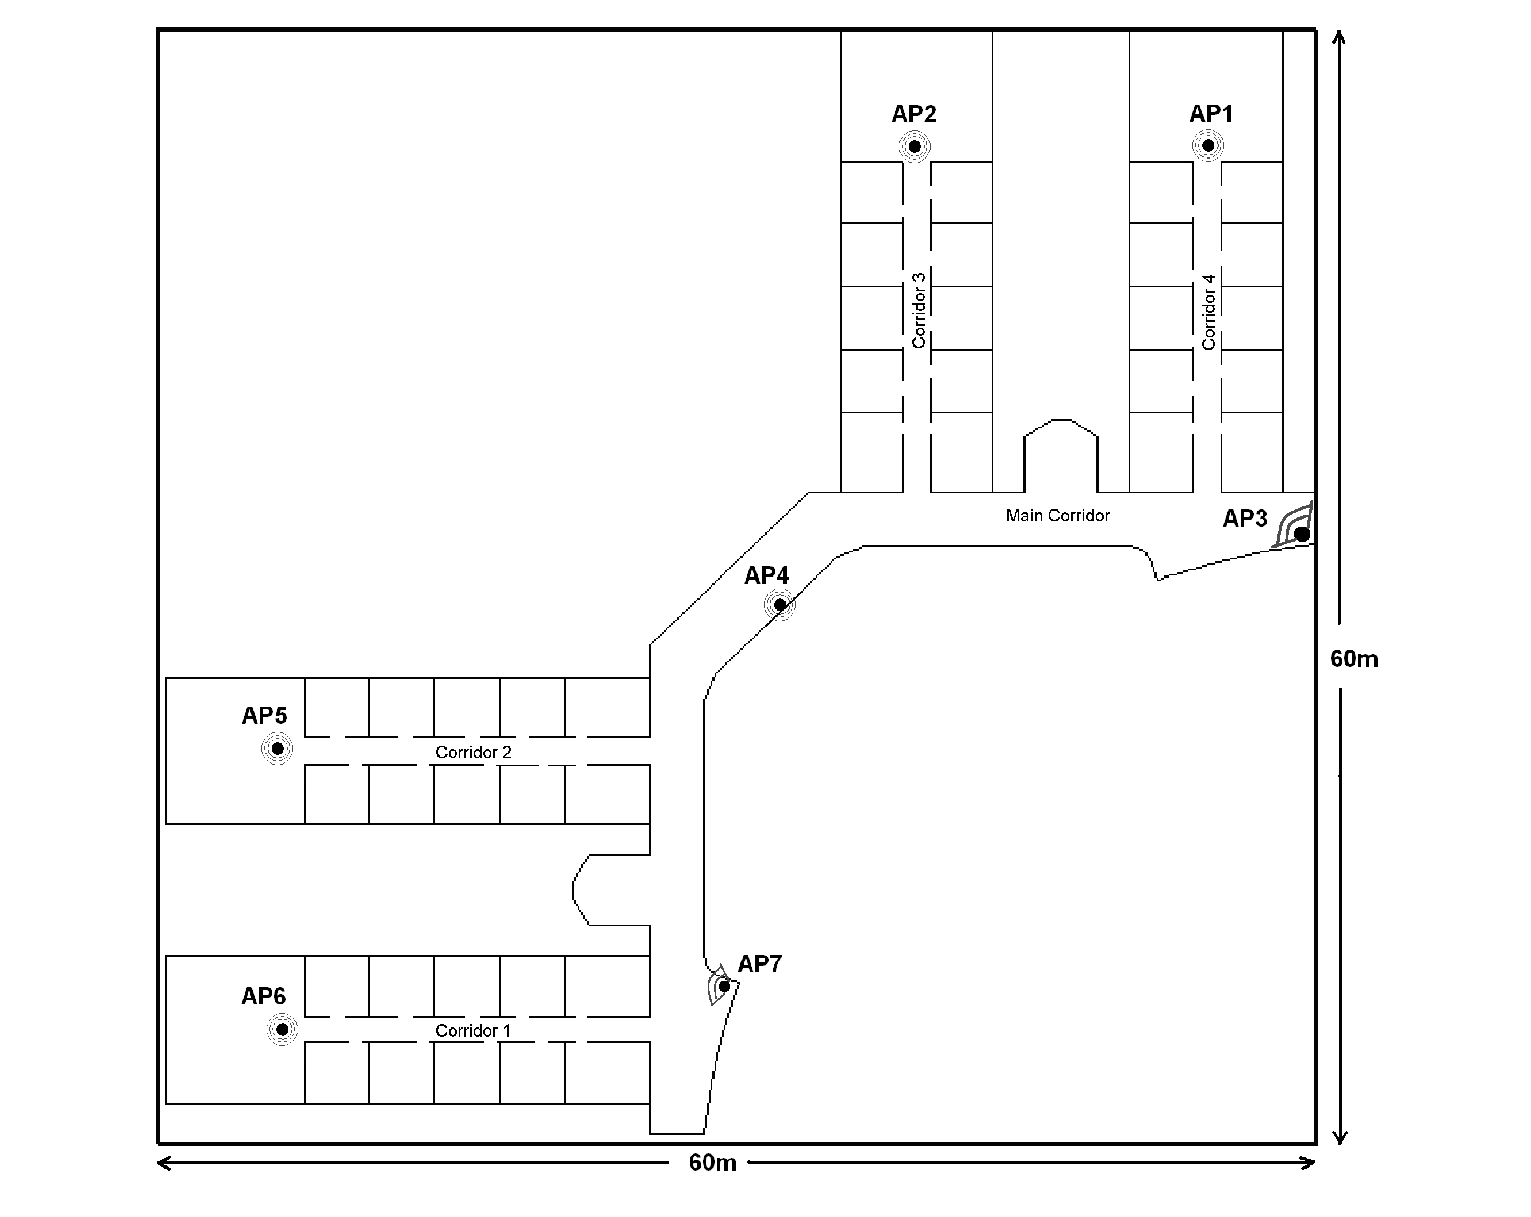
\includegraphics[width=4.7in]{Figure1}
  % where an .eps filename suffix will be assumed under latex, 
  % and a .pdf suffix will be assumed for pdflatex
  \caption{Departamento de Electr�nica.}
  \label{fig1}
\end{figure}

Y ahora un ejemplo en el que ponemos el \texttt{caption} en el lateral:

\begin{SCfigure}
  \centering
  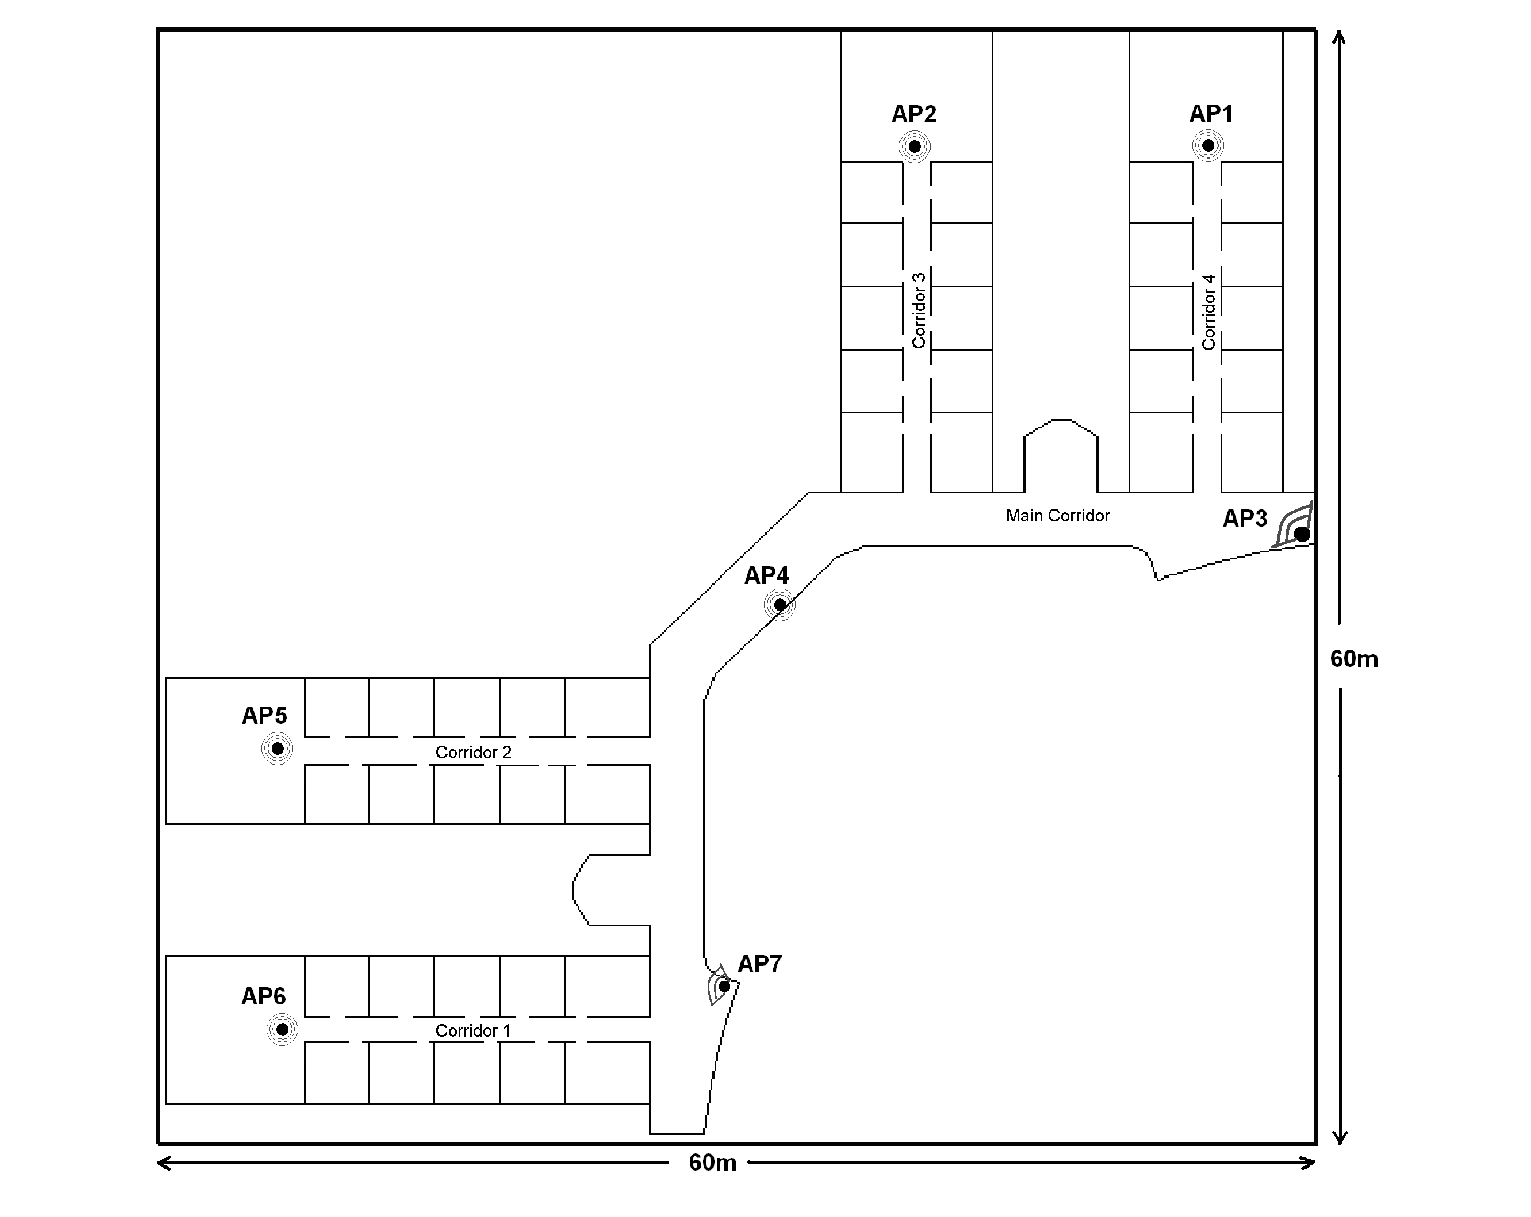
\includegraphics[width=0.5\textwidth]{Figure1}
  \caption{Departamento de Electr�nica en el lateral.}
\end{SCfigure}



\section{T�cnicas utilizadas}
\label{sec:tecnicas-utilizadas}

Aqu� vamos a probar todos los niveles de secci�n disponibles, para
evaluar la asignaci�n de \texttt{tocdepth}...

Blah, blah, blah\ldots


\subsection{Subsecci�n}
\label{sec:subseccion}


\subsubsection{Subsubsecci�n}
\label{sec:subsubseccion}

\paragraph{Paragraph}
\label{sec:paragraph-1}


\subparagraph{Subparagraph}
\label{sec:subparagraph}



\section{Conclusiones}
\label{sec:conclusiones-teoria}

Blah, blah, blah\ldots

%%% Local Variables:
%%% TeX-master: "../book"
%%% End:
